\documentclass[landscape]{article}

\setlength{\textheight}{190mm}
\setlength{\topmargin}{-29mm}
\setlength{\textwidth}{297mm}
\setlength{\oddsidemargin}{-23mm}

\usepackage{graphicx,url}
\renewcommand{\rmdefault}{pag}
\renewcommand{\sfdefault}{phv}

\newlength{\colw}
\setlength{\colw}{79mm}

\pagestyle{empty}

\newcommand{\column}[1]{\hspace*{9mm}{}
  \parbox[t][0.99\textheight][t]{\colw}{\parskip1ex
    #1\parskip0ex}\hspace{9mm}{}}

\special{landscape}

\begin{document}

\noindent
\column{
  \begin{itemize}
   \item \emph{``R \ldots\ is the best way to ensure portable, open code that
    is freely available to all interested users, with state-of-the-art
    algorithms for statistical calculations.''} (Scientific Advisory
    Panel, US Environmental Protection Agency)
   \item Implements S, which \emph{``has become a kind of lingua
      franca of statistical computing''} (J.\ Fox, 2002),
    that \emph{``\ldots\ has forever
      altered the way how people analyze, visualize and manipulate data
      \ldots''} (Association of Computer Machinery Software System
      Award 1998 to John Chambers)
   \item Compatible with S-Plus at the language level, data exchange
    with Excel, Minitab, SAS, SPSS, SQL databases, \ldots
   \item A means of rapid technology transfer through packages
   \item An embeddable extension language, interfaces to C, C++,
    FORTRAN, Java, Perl, Python, Tcl/Tk, \ldots
  \end{itemize}

  \vfill
  \begin{center}
    \footnotesize
    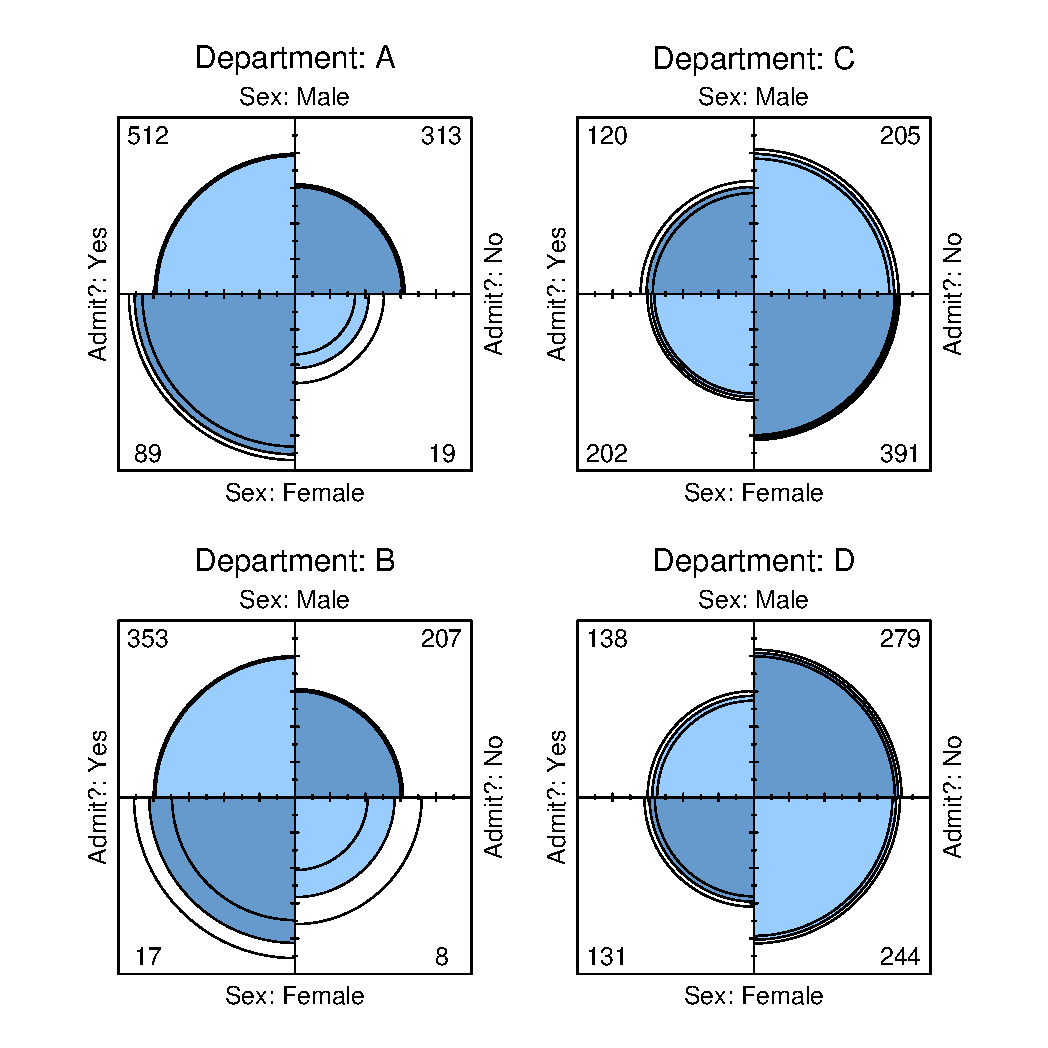
\includegraphics[width=0.9\colw]{fourfoldplot}
    \sf Berkeley admission data
  \end{center}
  }
\column{
  \begin{center}
    \footnotesize\sf
    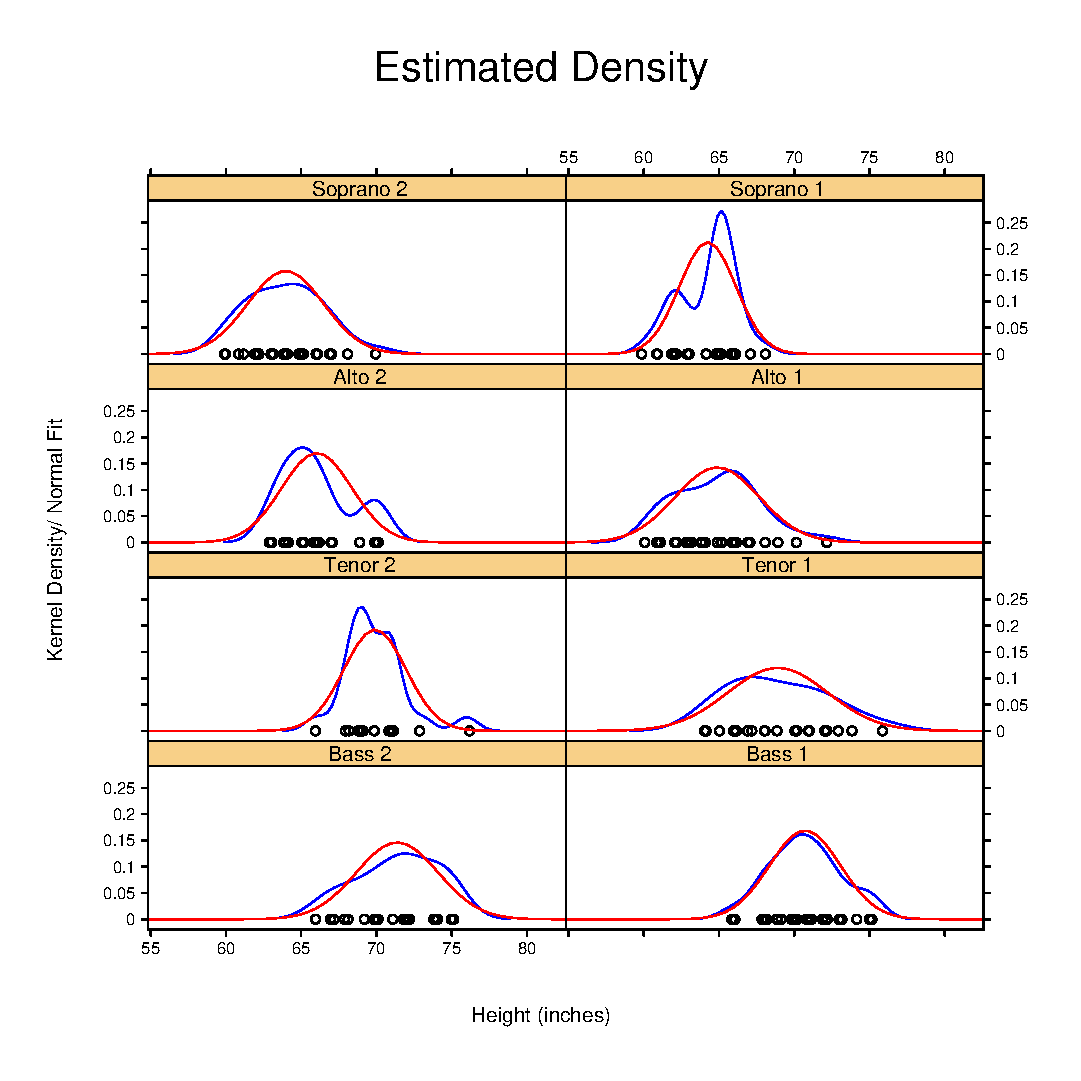
\includegraphics[width=\colw]{lattice-density}
    Singer heights grouped by voice part
  \end{center}

  \vfill
  \flushleft
  \begin{itemize}
   \item Classical statistical tests
   \item Generalized linear models
   \item Multivariate statistics
   \item Nonlinear mixed effects models
   \item Robust statistics
   \item Survival analysis
   \item Classification and regression trees
   \item Neural networks
  \end{itemize}
  \vfill
  Runs on all major platforms:\\
  Linux, Macintosh, Unix, Windows
  \vfill
  Just install it and try it:\\  Comes with a money-back guarantee.

  \begin{flushright}\tiny
   $\ $Date: 2003/04/11 11:26:09 $\ $
  \end{flushright}
}
\column{
    \vfill
  \begin{center}
    
\includegraphics{Rlogo}\\[2cm]
    \bf
    \Large
    Free Software for\\[1cm]
    \Huge
    Statistical Computing,\\ Data Analysis\\ \& Graphics\\[1cm]
    \Large
    \url{www.R-project.org}
  \end{center}
  \vfill
  }

\newpage
\noindent
\column{
  R, also known as ``GNU S'', is a language and environment for
  statistical computing and graphics. R implements a dialect of the
  award-winning language S, developed at Bell Laboratories by John
  Chambers et al. For newcomers it provides easy access to a wide
  variety of statistical and graphical techniques. Advanced users are
  offered a full-featured programming language with which to add
  functionality by defining new functions.

  \begin{center}\footnotesize\sf
    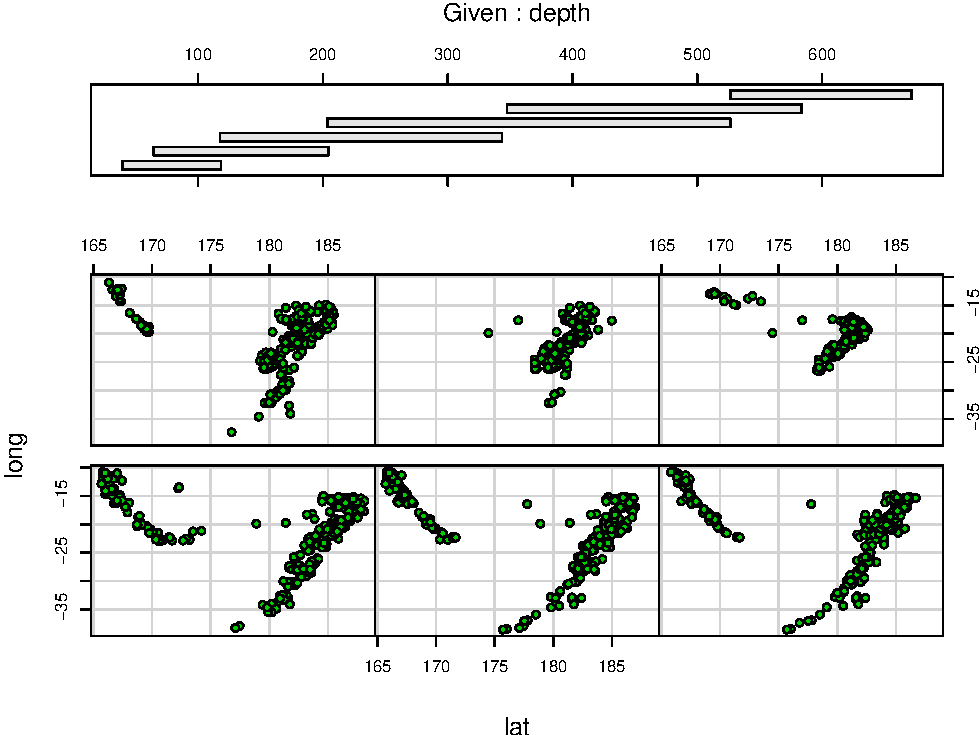
\includegraphics[width=\colw]{quakes-coplot}
    Locations of earthquakes near Fiji
  \end{center}

  R is easily extensible using a package library system and a
  wide-ranging and extensive set of contributed packages is available
  from the Comprehensive R Archive Network (http://cran.R-project.org
  and mirrors).  R is open source software and an official part of the
  Free Software Foundation's GNU project. Like Linux it is released
  under the terms of the GNU General Public License (GPL).

  Using open source software for data analysis makes truly
  reproducible research possible: Anyone interested can use exactly
  the same tools to repeat a study, without restrictions by
  hardware requirements or available software licenses.
  }
\column{
  \begin{center}
    \footnotesize\sf
    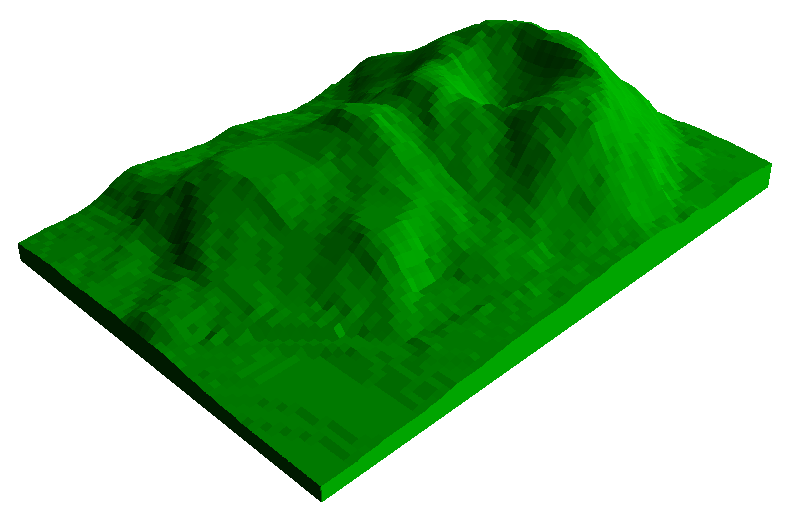
\includegraphics[width=0.85\colw]{volcano-persp}\\
    Perspective plot of Maunga Whau Volcano (NZ)
  \end{center}
  
  R was initially written by Ross Ihaka and Robert Gentleman
  (University of Auckland, New Zealand).  Since 1997 development has
  been in the hands of an international group (the ``R Core Team''):
  Douglas Bates (USA), John Chambers (USA), Peter Dalgaard (Denmark),
  Robert Gentleman (USA), Kurt Hornik (Austria), Stefano Iacus
  (Italy), Ross Ihaka (NZ), Friedrich Leisch (Austria), Thomas Lumley
  (USA), Martin M{\"a}chler (Switzerland), Guido Masarotto (Italy),
  Duncan Murdoch (Canada), Paul Murrell (NZ), Martyn Plummer (France),
  Brian Ripley (UK), Duncan Temple Lang (USA), and Luke Tierney (USA).
  In addition, there is a wealth of high-quality add-on packages
  provided by a very active development community.
  \begin{center}
    \footnotesize\sf
    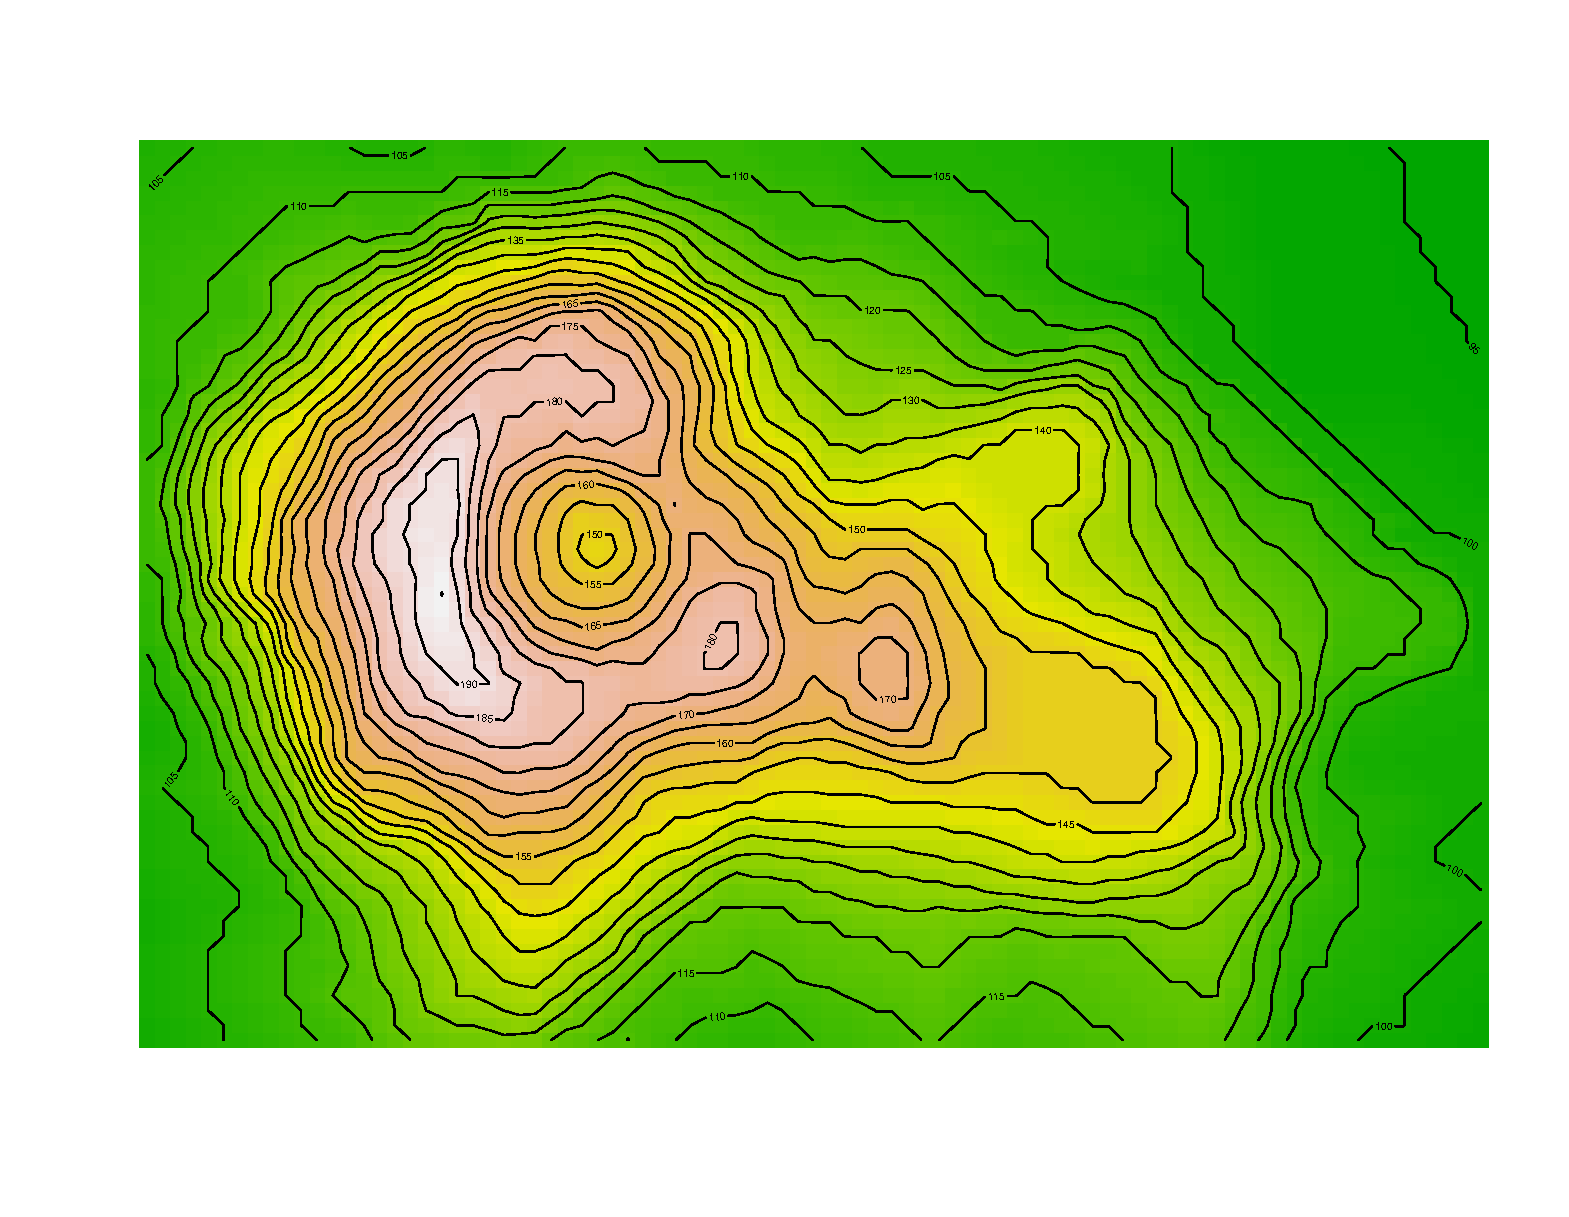
\includegraphics[width=0.85\colw]{volcano-image}\\
    Contour plot of Maunga Whau Volcano (NZ)
  \end{center}
}
\column{
  \textbf{The R Homepage}
  \begin{quote}
    \url{http://www.R-project.org}
  \end{quote}
  offers background information and lots of useful material related to
  R.

  \textbf{CRAN}

  The Comprehensive R Archive Network offers free download of the
  software and contributed extension packages both as sources and
  precompiled binaries. The master node in Vienna, Austria, can be found at
  \begin{quote}
    \url{http://cran.R-project.org}
  \end{quote}
  and is mirrored to places all around the world.

  \textbf{Manuals}

  R comes with a growing set of manuals: An Introduction to R, Writing R
  Extensions, The R Language Definition, R Data Import/Export, and R
  Installation and Administration. In addition several hundred help
  pages for all functions of R are available.

  \textbf{Mailing Lists}

  Several mailing lists are used for information exchange in the R
  community, ranging from help requests of novice users to passionate
  discussions on future developments of R itself. Subscription
  information and archives can be found on the R homepage.

  \textbf{R News}

  The newsletter of the R project is published three times a year
  online at CRAN and informs about all aspects of R. It lists new
  features of the latest release, gives short introductions to
  extension packages and the regular column ``Programmer's Niche''
  shows tricks that even seasoned programmers will appreciate.

  }
\end{document}

%%% Local Variables:
%%% mode: latex
%%% TeX-master: t
%%% End:
